\section{Eye parameters}
\label{sec:eyeparameters}

In order to understand in which way eye trackers can be useful for early ASD diagnosis, it is fundamental to define and operationalize the eye movements of interest which need to be measured. In the context of this thesis, all the measurements of variables (e.g. velocity, amplitude, etc) related to categories of eye movements (e.g. saccades, smooth pursuit, etc) are defined as “eye parameters”, in order to highlight their purpose of indicators of cognitive or motor differences between groups of subjects. The various eye parameters provide insights about the possible divergent development of the involved neural circuitry.

As \citet[pp. 2-5]{leigh2015neurology} summarize, there are different categories of eye movements, which are basically rotations of the eye globes aimed to position the image fairly steadily on the central foveal region of the retina (within 0.5 deg from the center of the fovea), where the photoreceptor density is greatest. Eye movements can be distinguished basing on how they support vision, their physiology and anatomy. The categories of eye movements are vestibular movements, visual fixations, optokinetic movements, smooth pursuit, nystagmus quick phases, saccades and vergence. Each functional class of eye movements is suited to a specific purposes and the classes are distinguished by different anatomical and neural circuits. Gaze-shifting eye movements, such as saccades, point the fovea towards the target. Gaze-stabilizing reflexes, such as smooth pursuit, keep the fovea of each eye pointed at the target whenever the head is moving.

Eye trackers can measure and record directly some of these eye movements, such as fixations and saccades, while for others a further computation is needed in order to describe them, such as smooth pursuit eye movements. Moreover, in addition to the movements of the eye globes, eye trackers can compute more eye-related events like the pupillary dilation and the eye blinks.
Each type of eye movement or event is then operationalized depending on its specific features (e.g. timing, velocity, accuracy) in order to allow the researchers to measure its characteristics.

Saccades, smooth pursuit eye movements and fixations are the categories of eye movement most extensively studied in ASD so far \citep{johnson2016review}, and therefore the ones which are of most interest for this study, since research provides enough material to try to build a framework on.

\citet[pp. 2, 170, 290]{leigh2015neurology} describe further these eye movements:
\begin{itemize}
    \item Fixations are eye movements aimed to hold the image of a stationary object on the fovea by minimizing ocular drifts, even though ocular tremor happens in order to prevent habituation.
    \item Saccades are rapid eye movements which shift the line of sight between successive points of fixation and which bring images of objects of interest onto the fovea. Saccades are characterized by fast acceleration to high velocity, followed by a quick deceleration of equal magnitude \citep{wilkes2015oculomotor}.
    \item Smooth pursuit movements are generated continuously in order to hold the image of a small moving target on the fovea, by keeping the line of sight congruent to the line of movement of the target. Visual smooth pursuit movements are slower and gradual \citep{wilkes2015oculomotor}.
\end{itemize}
In addition to these parameters, pupil dilation and eye blinks are discussed in literature and they will be described.

\cite{falck-ytter2013eyetrackingASD} provide a quick overview of how the oculomotor system develops in TDg children: at birth infants can direct their gaze throughout the environment primarily using saccadic eye movements (often performing several hypometric saccades). As infants grow older, saccade latencies decrease and fewer corrective saccades are needed. Around two months of age, infants can perform smooth pursuit with the frequent use of saccades to reposition the eyes on the target, and by four months of age they can track objects smoothly on the horizontal plane. Predictive tracking is visible between two and four months of age. The oculomotor system continues to improve over the first year of life. Vertical and two-dimensional tracking matures over the first years and saccade latencies decrease continuously during infancy and childhood. Basing on this overview, it should be possible to assess saccades and smooth pursuit after the first year of life of the children, as well as potential delays and deficiencies.

As \cite{wilkes2015oculomotor} discuss, studies show that high-functioning adults with ASD have relatively typical, if more varied saccade function, but abnormal visual smooth pursuit. Less has been done on children, and some patterns are not as clear as in adults.

Even though the number of retrieved articles researching with eye trackers on ASDg is high (as described in Chapter~\ref{chap:background}, the following sections had to be based on a rather low number of papers which provide detailed measurements of specific eye parameters. Moreover, not many studies investigating on specific eye parameters have been done on infants or toddlers at risk or who eventually have been diagnosed with ASD. Some of the studies reported as follows have been done on children belonging to an older age range, or even adolescents or young adults. This factor might not let the results of these studies to be fully valid for infants in early diagnosis range (defined here as between 12-24 months old), due to the children’s development over the months. However, these studies or reviews are the ones which studied subjects in the nearest age groups to the target one (or the studies were cross-sectional or longitudinal, including children), and which described in sufficient detail the ASD group characteristics. ASDg adults are a subject group potentially very different from infants or toddlers for obvious development reasons. However, evidences of abnormal eye parameters in older age might provide hints about earlier impairments which have not been treated by the education and the therapies which the subjects undergone during their lifetime.

In the next sections the various types of eye movements and parameters are described in detail, as well as their potential relation with early ASD diagnosis.



\subsection{Smooth pursuit}
\label{sec:smoothpursuittheory}

As \cite{takarae2004smoothpursuit} describe, smooth pursuit requires rapid, temporally precise integration of activity within several brain areas in order to visually track moving targets in the space, making studies of visual pursuit suitable for evaluating functional brain connectivity in ASDg. Neuroimaging studies highlight how the relevant brain circuitry includes the extrastriate areas of visual cortex devoted to the processing of visual motion information, cortical eye fields and cerebellum that are involved in translating sensory information to motor commands, and the striatum and brainstem which are involved in initiating motor commands.

As \cite{brenner2007visualsearch} summarize, smooth pursuit is a process which articulates on two phases: a first phase, called open loop, takes place in the first 100 ms after the presentation of the stimuli–which is the time that a pursuit eye movement take to be initiated \citep[pp. 298]{leigh2015neurology} –and the control of pursuit is almost exclusively dependent on sensory analysis of visual motion \citep{takarae2004smoothpursuit}. After this first phase, there is the closed loop phase of sustained pursuit, in which feedback, such as predictive or performance-based information, rather than an analysis of visual motion \citep{takarae2004smoothpursuit}, is used to update eye movement. Smooth-pursuit movements must me generated in response to local optic flow on the fovea but not on the rest of the retina, and this requires the brain to not process visual motion save for the one happening in the fovea \citep[pp. 290]{leigh2015neurology}. \cite{takarae2004smoothpursuit} explain that the prediction mechanism is fundamental since once a moving stimulus is tracked, its movement relative to eye velocity should become near zero, and therefore it provides insufficient information to drive further smooth pursuit. They also describe that the frontal eye fields and cerebellum are believed to play a crucial role during closed-loop predictive and performance-based pursuit, and abnormalities in the cerebellum are one of the most consistent histopathological findings in ASD. Cerebellum is believed to make a large contribution to the adaptation of smooth pursuit \citep[pp. 326]{leigh2015neurology}.

As \cite{wilkes2015oculomotor} describe, smooth pursuit eye movements have slower acceleration and velocity than saccades, and they cannot be performed in the absence of a moving visual stimulus. Two parameters are commonly studied:
\begin{itemize}
    \item Gain: maximum degree of displacement of the eye as compared to the maximum degree of displacement of the target visual stimulus;
    \item Phase lead/lag: mean degree of displacement by which the eye leads or lags behind the target stimulus. The less phase difference between eye and target, the more the smooth pursuit movement is accurate.
\end{itemize}

As \cite{kemner2004smoothpursuit} show, smooth pursuit gain can be computed as position gain (i.e. eye position as a linear function of the target position) or, more commonly, as velocity gain (i.e. how accurately eye velocity matches the velocity of a moving target \citep{johnson2016review}). Neither fixations nor smooth pursuit eye movements physiologically can have a velocity higher than 100 deg/s \citep{larsson2015detection}.

\cite{vonhofsten1997smoothpursuit} conducted a study which illustrates how smooth pursuit tracking develops in TD infants, and which serves as a basis in order to understand if and how ASDg behaves differently.
They measured eye (saccades and smooth pursuit) and head movements in 11 healthy and full-born TDg infants at 2, 3, and 5 months of age, through EOG (Electro-oculography, 200 Hz). The gaze was estimated as the sum of eye and head positions. The subjects were presented with a sinusoidal and triangular target moving horizontally by different amplitudes (12.5 deg or 25 deg of visual angle) and frequencies (0.2 Hz and 0.4 Hz) (Fig.~\ref{fig:sinetriangle}). Saccades were detected when the eye velocity was higher than 50 deg/sec of the tracking velocity amplitude, and they were eliminated from the composite eye movement record, in order to obtain two different set of records, one for the smooth pursuit movements and the other for the saccades.
Regarding smooth pursuit development, they observed that all the infants displayed some smooth eye tracking. Smooth pursuit gain increased with age: at 2-3 months, the lag of the smooth pursuit was small for the sinusoidal motion but large for the triangular one. These differences might be due to a velocity-based local analysis process in the infants, which works better for prediction of the continuous sinusoidal motion but not for the abruptly changing triangular motion, preventing accurate predictive tracking. They found a higher proportion of smooth pursuit at the lower amplitude and frequency. The authors suggest that the ability to track sinusoidal motion emerges some time between 1 and 2 months of age.
At 5 months tracking become clearly more predictive: smooth pursuit was leading the sinusoidal motion and the lag for the triangular one was small. Head tracking increased substantially with age and its lag was always large.
Head always lagged the target by at least a quarter of a second on average, which suggests that prediction does not affect head tracking. Head gain increased significantly over the time and consequently the gain of eye movements decreased. Eventually, the coupling between head and eye movements always allowed for the pursuit gain to be close to 1.
Regarding saccade development, they observed that saccades occurred regularly and often came in bursts at the higher velocity parts of the motion. Saccadic amplitude varied as a function of target velocity. The triangular motion elicited a higher number saccades, of wider amplitude and frequency than the sinusoidal one. At 5 months, the relative proportion of saccades was similar to the one present in adults.

\begin{figure}[h]
  \centering
  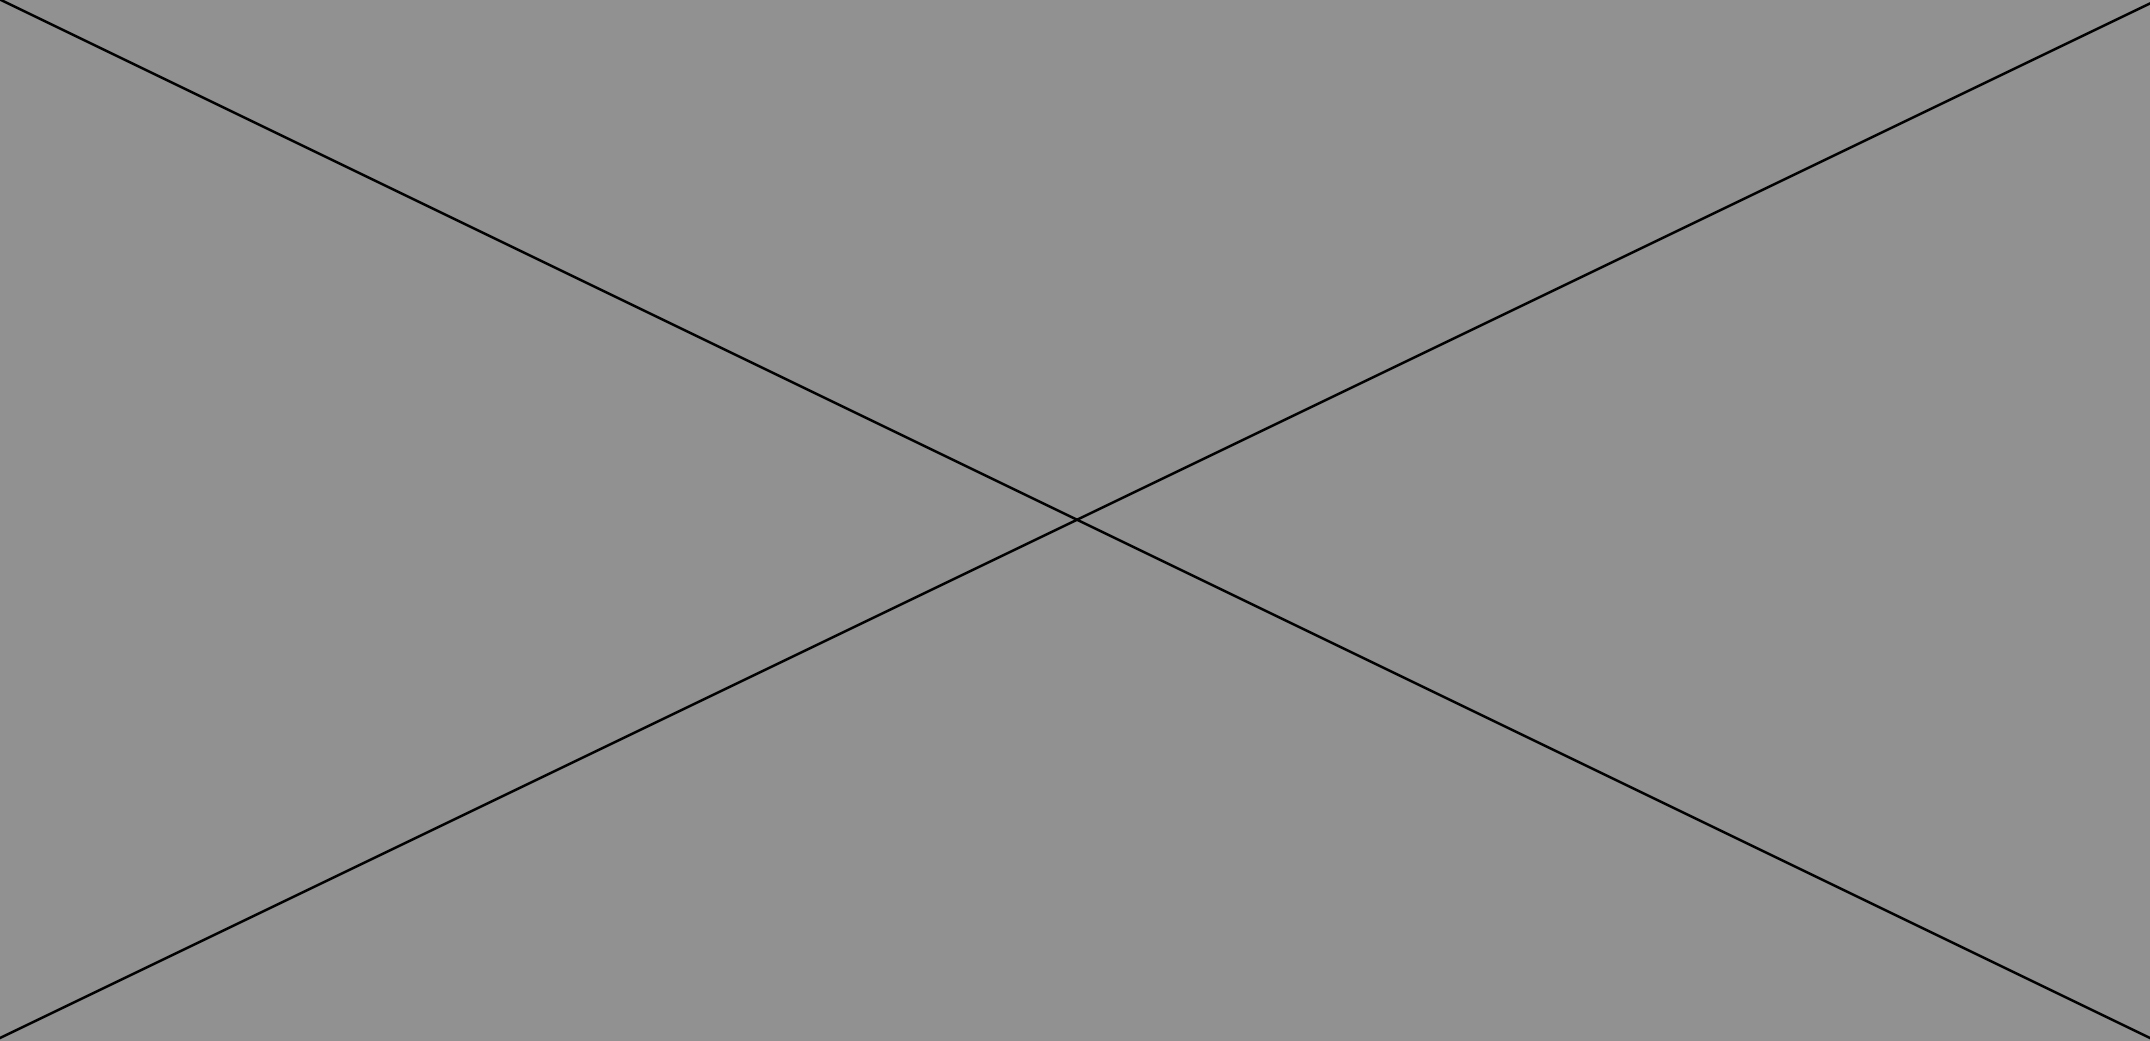
\includegraphics[width=.5\textwidth]{figures/placeholderImg.jpg}
  \caption[sinusoidal and triangular motion]{Smooth eye pursuit visualization of sinusoidal and triangular motion stimuli. Images retrieved from \cite{vonhofsten1997smoothpursuit}.}
  \label{fig:sinetriangle}
\end{figure}

ASDg seem to show significative abnormalities in smooth pursuit movements. \cite{johnson2016review} reviewed results from studies reporting open loop gain measurements (on a total of 101 ASDg and 140 TDg) and closed loop gain measurements (on a total of 114 ASDg and 154 TDg) finding strong evidences for significant deficits of pursuit gain in both open- and closed-loop phases of pursuit eye movements in ASDg. Even though the authors state that these results are one most robust indicators of smooth pursuit impairments, the subjects of the reviewed studies had a mean age ranging from 16.3 and 24.5 years old, and therefore they were either adolescents or adults.

\cite{takarae2004smoothpursuit} compared pursuit eye movements of 60 high-functioning ASDg (children, adolescents and adults, mean age 20.05 years old, SD 11.24) and 94 TDg using foveofugal step-ramp, pure-ramp and oscillating target tasks. They observerved that ASDg showed normal pursuit latency, but reduced closed-loop pursuit gain in all the tasks (which was consistent and not increasing across target speeds), and these abnormal parameters become more evident after mid-adolescence (>16 years), suggesting a reduced development of the pursuit system  (Fig.~\ref{fig:pursuitASDg}). ASDg also showed lower open-loop pursuit gain in the initial catch-up saccades during a foveofugal step-ramp task, when the targets moved into the right visual field. This lateralized effects was more pronounced in younger ASDg. 
Lower open-loop gain suggests disturbances in the transfer of visual motion information from sensory to sensorimotor systems, which affects the fidelity or resolution of visual motion information, but not the speed through which the information is transferred, since open-loop latency was comparable to TDg.
The authors suggest that the reduced functional connectivity within the visual pursuit system–which is caused by disturbs in the development of the brain like the possible disruption of open-loop pursuit in the right hemifield and involving the cerebellum, and the possible developmental failure in the sensorimotor systems mediating closed-loop pursuit–appears to be a fundamental characteristic of ASD.

\begin{figure}[h]
  \centering
  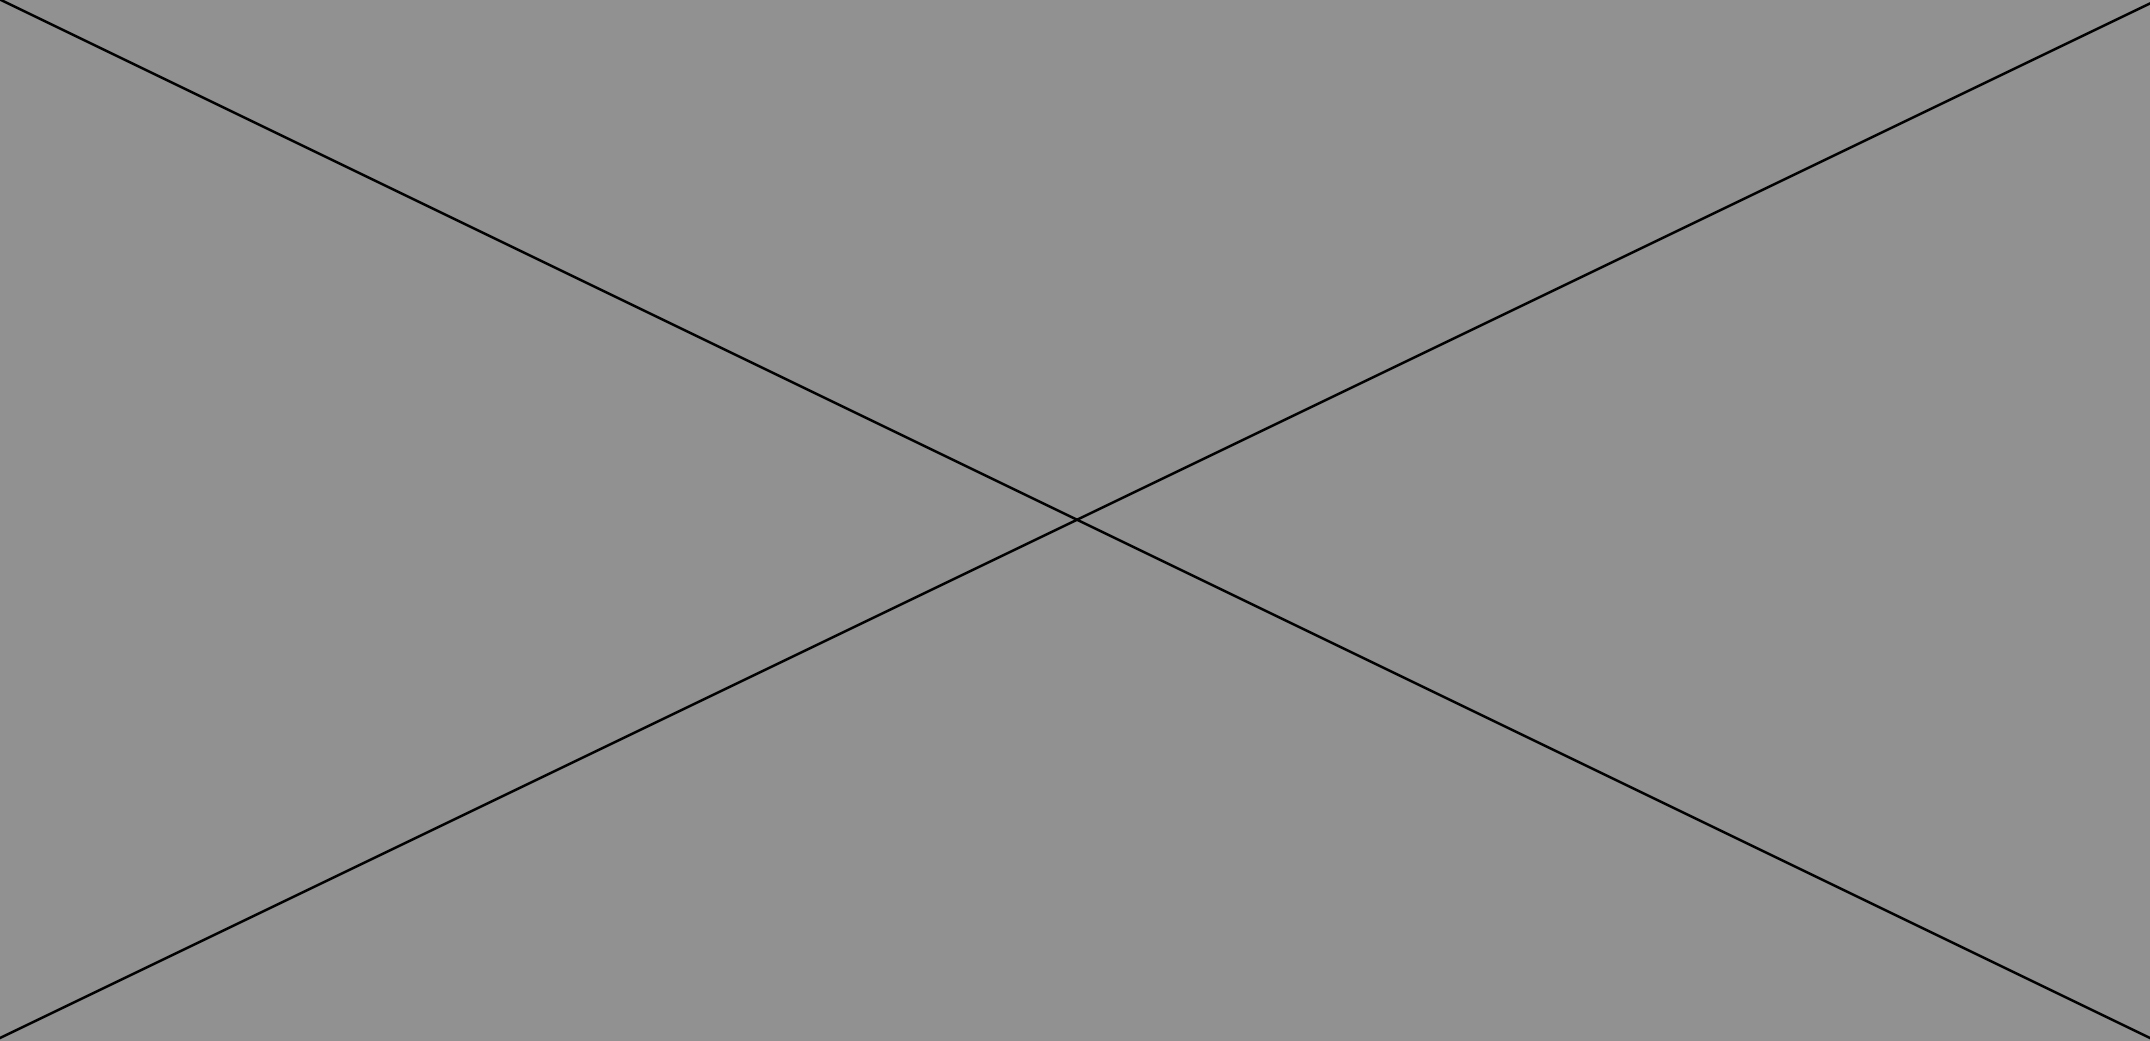
\includegraphics[width=.5\textwidth]{figures/placeholderImg.jpg}
  \caption[pursuit measurements ASDg]{Diagrams from \cite{takarae2004smoothpursuit} showing differences between ASDg and TDg smooth pursuit performance. This study was also included in the review from \cite{johnson2016review}.}
  \label{fig:pursuitASDg}
\end{figure}

Even though smooth pursuit parameters seem to be discern ASDg from TDg in a reliable way, there are some contrasting results in literature.

\cite{wilkes2015oculomotor} investigated on saccade and smooth pursuit performance in 16 high-functioning ASDg children between 6 - 12 years old (mean age 104 months, SD 23, IQ > 70) and 24 TDg. They used VOG goggles (I-Portal/Neuro-Kinetics, 100 Hz) to record eye movements while presenting a red laser-light as stimuli in a dark room. The stimuli moved both on an horizontal and vertical axis. They observed that ASDg had significantly lower mean smooth pursuit phase for vertical smooth pursuit at .10 Hz (where pursuit is typically more accurate) with a trending group difference at 0.50 Hz, but no differences in mean gain or phase for horizontal smooth pursuit conditions. They observed greater variance horizontal smooth pursuit phase in ASDg. They argue that the more evident difference in group means for phase in vertical, but not horizontal conditions, can be related to the relatively infrequent use of visual pursuit in the vertical plane, since in daily experience tracking objects continuously in the vertical plane is more rare than tracking objects in the horizontal plane. Differences in phase implies that the fovea is not on target but in the periphery.

\cite{vonhofsten2009lookingevents} made a study on 10 ASDg children, between 3 to 6 years old (mean age 4:8 years, range 2:10–6:1 years) compared to 1 and 3 years old TDg, evaluating their ability to track an object with smooth pursuit and their ability to anticipate the reappearance of a temporarily occluded moving object, looking for indicators of impaired motion perception or predictive ability. They used cornea reflection eye tracking (Tobii 1750/Tobii Technology, 50 Hz).They observed that ASDg tracked a sinusoidally moving object with no significant lag and with the similar smooth pursuit gain as TDg. The authors acknowledge the contradiction with previous results in literature, which reported deficient motion perception in ASDg, by speculating that it could be possible that ASDg are deficient in their ability to integrate local motions into coherent wholes but not in their ability to track single motions. ASDg also shown to be able to anticipate the reappearance of the temporarily occluded moving object. However, these results cannot be fully compared with other papers, since the sampling frequency of the eye tracking equipment was rather low to have precise measurements of saccade and smooth pursuit movements. \cite{smyrnis2008guidelines} advices to use sampling frequencies of at least 200 Hz for saccade and smooth pursuit measurements, while here the authors used only 50 Hz.

Acknowledging the findings in literature of abnormalities in smooth pursuit eye movements in ASDg, \cite{kemner2004smoothpursuit} investigated on smooth pursuit in the group of children with the more generic diagnosis of pervasive developmental disorder (PDD) in order to assess the presence of endophenotypic markers of general genetic factors predisposing for psychopathology. They observed 16 children (9 diagnosed with PDD, 7 diagnosed with ASD, mean age 10.9 years old, SD 2.0) and 18 TDg during smooth pursuit task and and 14 children (7 diagnosed with PDD, 7 diagnosed with ASD, mean age 11.1 years old, SD 2.1) and 15 TDg during visually guided saccade tasks. They used electro-oculography (EOG, 85 Hz, nine points calibration) to record the smooth pursuit eye movements while displaying a target moving at a constant velocity in triangular motion, and horizontal and vertical saccade tasks.
In smooth pursuit, they found that position gain decreased significantly at target velocities greater than 16 deg/s and that the number of saccadic intrusions increased at target velocities between 8 and 24 deg/s and then assessed at around 2.7 saccades/second.
In saccades, amplitude, scatter in amplitude, duration and peak velocity increased significantly with increasing amplitude between the targets.
No differences in smooth pursuit or saccade parameters were found between the groups, indicating that eye tracking is normal in children with PDD (and reached maturation to a normal levels in children with PDD of about 10 years of age), suggesting that smooth pursuit eye movements are not a neurophysiological marker of PDD. Their findings of normal of smooth pursuit eye movements are not consistent with the literature presented above \citep{takarae2004smoothpursuit,johnson2016review}. As also the authors acknowledge, in this study the sample was a mixed group of children diagnosed with PDD and ASD. The high variability of condition of the children and the also small sample could have lead to a high variability in the results. Moreover, the level of noise in the EOG system might have influenced the results, which might not be fully comparable to the measurements done by other studies with high-frequency IR eye tracking (as discussed also in the previous paragraph for \citealp{vonhofsten2009lookingevents}).


\subsection{Saccades}
\label{sec:saccadestheory}

As \citet[pp. 170-171]{leigh2015neurology} summarize, abnormalities of saccades are often distinctive and highlight disorders of specific mechanisms, and they can describe aspects of cognition such as memory, attention, motivation, reward, prediction and decision making, as well as neurological and psychiatric disease. There are several types of saccade movements, but basically they can be grouped in two macrocategories: volitional (i.e. made as part of purposeful behavior) and reflexive (generated by novel visual, auditory or tactile stimuli, which unexpectedly occur within the environment). Saccades do not last much longer than 100 milliseconds, which is about the time it takes for new information to be processed by the visual system and transformed into a new motor command.

\cite{brenner2007visualsearch} summarize several parameters which can be computed from saccades:
\begin{itemize}
    \item Amplitude: the size, or angular rotation, of the saccade.
    \item Duration: the time taken for the eye to reach the target. The duration of a saccade is approximately linearly related to their amplitude for amplitudes between 1 deg and 50 deg \citep[p. 172]{leigh2015neurology}.
    \item Latency: the time which elapses between the appearance of the target and the onset of a saccade in response to that target. As \cite{smyrnis2008guidelines} summarizes, saccades can be defined accordingly to their latency (in milliseconds): anticipatory saccades ( \(\leq\) 80), express saccades (80 \textless x \(\leq\) 120), fast regular saccades (135 \(\leq\) x \textless 180), slow regular saccades (180 \(\leq\) x \textless 400) and late saccades (400 \(\leq\) x \textless 700). 
    \item Accuracy: how precisely the saccade directs the fovea to the target, by executing saccades of correct amplitude \citep{pensiero2009saccades}. It is determined in relation to the expected saccade amplitude: insufficient (hypometric) or excessively high (hypermetric). Saccade gain is an index of saccade accuracy, and it is described as the ratio between target displacement and saccade displacement \citep{johnson2016review}.
    \item Peak velocity: as \citet[pp. 171-172]{leigh2015neurology} describe, peak velocity is the top speed of the saccade. The relationship between amplitude, duration and peak velocity is consistent enough in humans, and it is defined as main sequence relationship. Saccades which differ from the main sequence can be seen as an indicator of abnormal behavior. For saccades lower than 20 deg of amplitude, the relationship between amplitude and peak velocity is linear, while for larger amplitude saccades the peak velocity saturates and flattens itself. Through the main sequence it is possible to investigate the working of the premotor system (if the burst cells producing the recorded saccade correctly, independently of the direction, amplitude and timing) \citep{pensiero2009saccades}.
\end{itemize}

As \cite{pensiero2009saccades} describe, saccades are basic components of the oculomotor system and they are already present in infancy. If saccades are impaired, they could affect the development of sensorimotor, attentional, and cognitive functions of the infants. For example, saccades can help in investigating on brainstem, which is considered to be the center of eye movement (and saccades in particular) generation.

Literature presents contradictory findings about abnormal saccadic eye movements in ASDg, even though there seem to be evidences of impairments. Some studies report lower peak velocity in autistic children, other no differences in terms of accuracy, velocity, or latency, others saccadic dysmetria consistent with reports of histological abnormalities in the cerebellum. \cite{freedman2017biomarkers} suggest that differences in the structure of the cerebellum in ASDg could critically impact visuo-sensorimotor development in early infancy. Saccade adaptation and accuracy can be seen as a good candidate metric of different functioning of the cerebellum in ASD or in other developmental disorders, and these metrics can be assessed in children as young as 10–41 months of age.

However, in their review, \cite{johnson2016review} found that mean peak velocity, mean latency and mean accuracy (computed though gain) of saccades seem to not significantly differentiate ASDg from TDg, suggesting that ASDg does not show significant impairments in shifting and orienting visual attention as well as controlling and sustaining fixation. However, in part of the studies investigating saccades (on a total of 93 ASDg and 147 TDg, mean age of ASDg ranging from 11.2 to 20.5 years old, mean IQs above 95.9 points), ASDg show consistently a significant greater variable error of saccades (standard deviation of saccade gain), which indicates saccade dysmetria (i.e. the tendency of overshoot or undershoot the target) in visually guided saccades tasks with target amplitudes ranging from 5 deg to 30 deg.

\cite{pensiero2009saccades} investigated saccades in ASDg children 14 ASDg children (5 to 12 years old, mean age 8.1 years old, high severity, IQ > 60) and in 20 age matched TDg, in order to assess possible alterations of saccades at an early stage. They used an eye tracker (500 Hz) to collect data about amplitude, duration, latency and peak velocity, in order to compute main sequence relationships. They used LED lights targets blinking in random positions on an horizontal axis, avoiding to use social stimuli in order to measure only the features of the generation of saccadic movements. They kept the head of the children on a chin rest.
Eventually, only 1 ASDg participant showed abnormalities of the main sequence. The others did not show clear alterations of the saccadic features. However ASDg produced more blinks before and during fast eye movements, shown tracts of saccadic initiation failure and changes in the saccadic velocity profiles (which happened 37\% of the times at 20-25 deg amplitudes, compared to the 18\% of TDg) that could be due to an alteration of the brainstem.
It has to be noted that the kind of experiment setting used by the authors might not be suitable for early ASD diagnosis on very small children. They indeed tested older children, who were also able to be continuously prompted to follow with their gaze the illuminated LEDs. This kind of verbal prompting might not work on infants. However, their results suggest that, if there could be alterations in small children’s saccades, they might get compensated over the time during development.

At the moment it seems that the saccadic parameters involved in the main sequence do not differentiate clearly ASDg from TDg, However, some secondary parameters, like the standard deviation of saccade gain, seem to be consistent and a reliable predictor of ASD.


\subsection{Fixations}
\label{sec:fixationsstheory}

Fixations are identified when the point of gaze remains within 1 degree of visual angle for at least 100 milliseconds \citep{boraston2007eyetrackingASD}.

As \cite{johnson2016review} describe, overall fixation parameters in ASDg are comparable to TDg, however it presents disturbs in stabilization and fixation maintenance, highlighted by a more variable amplitude of microsaccades. Moreover, ASDg seems to not be characterized by enhanced visual processing.

As \cite{pensiero2009saccades} summarize, eye tracking technology has been used in investigations on the strategies used by ASDg during tasks involving social information processing. The most common stimuli used for investigating social attention in ASDg are pictures of human faces, but videotapes of social interactions, human voices, and abstract animations have also been employed.

Usually, in order to compute social attention from eye tracking, areas of interest (AOI) are identified in the stimuli prior to the tests. ASDg seems to significantly spend less time fixating social features of faces, like the eyes \citep{papagiannopoulou2014review, boraston2007eyetrackingASD}. The review from \cite{chitategmark2016socialattention} indicates that the lack of attention on social content in the stimuli, measured by fixation time on social AOIs, seems to be a significant predictor of ASD, and that these difficulties seem to not be affected by age or IQ, but to be a core feature of ASD.

However, defining which AOIs are identifying social contents within a visual stimuli is an arbitrary operation that is strongly related to the ecological validity and above all to the construct validity of eye tracking methodologies for ASD detection, as explained in detail in Section~\ref{sec:fwkvalidity}. Presenting a video or a picture on a screen, containing some arbitrarily defined social content, could potentially elicit in the children very different oculomotor responses than the ones they would perform in a natural setting, Highly controlled laboratory settings impact on the social relevance of the experimental stimuli \citep{papagiannopoulou2014review}, and the validity of defining social AOIs as parts of face and body (e.g. eyes or mouth) or the entire figures of people in the visual stimuli is highly dependent on ecological validity.

As a consequence of the different definition of social contents in studies stimuli, literature show contradictory findings, in particulars when children with ASD are the experimental subjects.

In the experiments from \cite{vonhofsten2009lookingevents}, 3 to 6 years old ASDg looked at the social AOIs (faces of the people involved in a conversation) in a video for less time than 1 year old and 3 year old TDg children. However, in the same experiment, ASDg looked at turntaking objects (a video showing objects emitting sounds and moving like if they were having a conversation) in a similar way of TDg, suggesting that ASDg did not have a general attention deficit but that they were less attracted by the social component of the conversation. 

The study from \cite{young2009gazechildren} suggests that even if there seems to be potential for using fixation towards social AOIs as index of potential ASD development in children, this potential seems to lose predictive value within the first 24 months of life. They conducted a longitudinal study on the gaze behavior of a group on infants at risk for autism with the objective of assessing the diagnostic reliability of the results from of one of their previous study \citep{merin2007fixation}. In their previous report, a group of those 6 months old children at risk shown an overall decreased amount of gaze to the mother’s eye region during a mother-child live interaction. The infants at risk looked less at the mother’s eyes. Those results highlighted how this kind of ASD symptoms seem to be present at very early stages of development. However, \cite{young2009gazechildren} affirm that the lack of visual attention to the eyes or a lack of shared affect during the first year of life might be related more to risk-status than to diagnostic outcome and may ultimately have poor specificity and poor clinical utility, since the majority of infant siblings of children with autism will exhibit typical development. The authors visited and collected infant behavior and eye tracking data (using a Tobii corneal-reflection eye-tracker, 30 Hz, five point calibration) on a final sample of 49 infants, who were visited at 6, 12, 18, and 24 months of age. AOIs were used to code each fixation frequencies and durations on eye, mouth, and other face regions. Eventually, out of the 49 infants only 3 were diagnosed with autism (1 from the low-risk sibling group, and 2 from the high-risk sibling group). All these 3 infants showed a high proportion of fixation to the eye region and did not exhibit any abnormal face scanning patterns at 6 months. Summarizing, the differences in fixation behavior at 6 months did not predict the development of ASD. 

\cite{vandergeest2002humanfigures} used an eye tracker (Iview Remote / SMI, 50 Hz, nine-point calibration) in order to investigate on fixation (latency, number and time) and scan path length behavior of high-functioning ASD children, in an older age group than \cite{young2009gazechildren} (mean age 10.6 years, SD 2.1 years). The stimuli were cartoon-like scenes that included neutral objects and a human figure. Their results indicate that fixations on human figure of ASDg was comparable to age- and IQ-matched TDg, suggesting that ASDg does not process socially loaded visual stimuli in a different way, even when they grow up. All the children looked longer and more often to the human figure than to the neutral objects, took the same time to first fixate the human figure and put the same effort in inspecting the pictures. Even though the experimental setting lacked ecological validity (it was not a real time interaction between humans in the environment) and the stimuli (full-color cartoon-like images) probably lacked social validity, still all the children looked more at the human figure than other parts of the scene, attributing them some special or social meaning. The authors suggest that abnormal gaze patterns in ASDg everyday life is not related to the nature of the visual stimuli but that other factors, like social interaction, may play a decisive role.

From these studies, it is evident that eye tracking studies on fixations on social vs. non-social stimuli can yield very different results. Moreover, a series of practical reasons would make the eye tracking measurements on fixations impractical.

Clinicians already assess the “social gaze” in their behavioral tests, in a rather complex situation like the shared play between the child and the evaluator (Minichiello S., personal communication). Possibly, the measurements on the gaze behavior with an eye tracker should be done in such kind of rich and playful environment in order to simulate an accurate gaze behavior in the children. However, this kind of experiment would imply to use mobile wear-on eye trackers on the children, since their head movements need to be not constrained and they need to be free to look ad interact at 360 deg in the environment. This kind of equipment might not be suitable to be used on very small children, or toddlers. Putting a device on the face or on the head of the child implies biasing their behavior to some extent, especially if they never worn a pair of glasses before.

Moreover, the video footage and the eye tracking data need to be checked manually by the evaluators or by using a rather complex video analysis software, in order to code the AOIs in such a dynamic environment. This kind of heavy post-test analysis might not suit the purpose of aiding the diagnosis process, letting it become even more bulky and expensive and causing attrition towards the technology itself.

An experimental setting in which the child is required to watch to a screen is less ecologically valid than presenting the child some stimuli in a playful environment. However, it could allow to perform quicker data analysis, since the stimuli are presented in a controlled environment and the software can compute AOIs or eye parameters in the same way for each testing.

Due to all these reasons, fixations will be not investigated further by the eye tracking framework developed for this study. The focus will be more on saccades and smooth pursuit parameters, which can be measured in detail in an experiment with controlled setting, in which ecological validity should not impact significantly on the measurement of these basic oculomotor functions.

The choice of not investigating further on fixations is explained even further in Section~\ref{sec:fwkvalidity}.



\subsection{Eye-related events}
\label{sec:eyerelatedevents}

Current eye trackers, as for example the SMI RED250mobile used in this study, have algorithms which can detect pupillary responses and eye blinks along with eye ball movements. These further parameters can provide information about emotional reactivity to stimuli and signs of rapport between conversational partners. ASDg seem to show reduced pupillary responses to non-conscious emotion processing and to visual stimuli \citep{nuske2014pupil,martineau2011pupil} and difficulties in synchronizing eye blinks with another speaker \citep{nakan02011blinks}.

However, since there are not many studies investigating these eye related events and that their measurement is impractical to be added in an eye tracking procedure for early ASD detection, these eye parameters are not added in the eye tracking framework.

\subsubsection{Pupillary responses}
\label{sec:pupillaryresponses}

As \cite{nuske2014pupil} describe, pupillary responses seem to be a reliable marker of emotional arousal and they are known to be functionally linked to the amygdala, allowing for comparisons with neuroimaging studies. \cite{martineau2011pupil} add that pupil size assessment has been used to evaluate neurological functioning, alertness, cognitive functioning and information processing, and it seems to be more reliable and sensitive than other autonomic measurements.

\cite{anderson2006visualscanning}, investigated visual scanning and pupillary responses to face and non-face stimuli, by using an eye tracker (ASL 504 / Applied Science Laboratories, the authors do not state the sampling frequency, five-point calibration) on 6 ASDg and 9 TDg children (age range 12 to 72 months, mean age 49.6 months). The stimuli consisted of colored photographs of children’s faces, animal faces, toys and landscapes, and they computed AOIs (in order to determine time tracked, duration of fixations, and average duration of fixations) and average pupil size for stimulus and interstimulus slides. They observed that ASDg showed significant lower time tracked, total time fixating, and average duration of fixations only for the landscape stimulus, which also contradicts findings in literature of reducing scanning to people’s faces (which is considered to be an indicator of social content). ASDg showed pupillary constriction to the overall and internal region of the children’s faces stimuli, while TDg showed dilation. ASDg showed similar pupillary responses to non-face stimuli (landscapes and toys). Therefore in their study, scanning measures to the landscape stimulus and pupil dilation on children’s faces stimulus significantly differentiated the ASDg from TDg. Due to the inconsistent results with literature for the visual scanning (as also already discussed in Section~\ref{sec:fixationsstheory}), the authors argue that pupillary responses might be a more sensitive indicator of ASD, and which is worth investigating further this parameter on infants with familial risk for ASD.

\cite{martineau2011pupil} conducted a study which seems to confirm the hypothesis that pupil measurements can provide useful information for discerning ASDg to TDg even in children belonging to an older age group than \cite{anderson2006visualscanning}. They recorded with an eye tracker (FaceLAB, 58.82 Hz) the mean pupil size and pupil waveform (average pupil size computed every 25o ms and then plotted over time) during a visual scanning task of still color photographs showing neutral faces, virtual faces (avatars) and objects, and the black slides separating the photographs (in order to test differences between dark and light conditions). The subjects were 19 children with ASD (mean age 118 months, ranging between 41 and 181 months), 19 mental age-matched TDg (mean age 87 months; range 44-178 months) and 19 chronological age-matched TDg (mean age 118 months, range 41-136 months).
The mean pupil size was significantly smaller in ASDg than in both TDg, both during the presentation of black and all the different stimuli slides with pictures. Pupil size correctly classified in 89\% of the participants in the ASD group, in 63\% in the mental age-matched TDg in 63\% in the chronological age-matched TDg. The mean pupil size in ASDg was significantly higher when seeing the picture stimuli compared to when they were seeing the black slides, while TDg showed opposite behavior.
Saccade waveforms were significantly different between ASDg and TDg when analyzing individually group, stimulus type and time, but not when analyzing together group - time - stimulus, meaning that overall the saccade waveform does not differ totally in the two groups.
ASDg mean pupil size was significantly higher when the stimuli were faces compared to objects, but not to avatars. Changes in pupil waveforms did not vary according to the stimulus used.
Both TDg showed significantly higher mean pupil size when when the stimuli were faces than when they were objects, but not when they were avatars for mental age-matched TDg.
While analyzing the changes in pupil size as a function of time, no significant difference emerged between groups, indicating that the modulation of pupil changes does not differ between ASDg and TDg. The pupil waveform varied according to time, highlighting three phases of pupil response: a first rapid dilation (< 1 s, indicating a change of perception), a second rapid constriction (< 1 s, a photo-motor reflex) and a third slow increase in pupil size (starting from ~1.25 s, the analysis of the stimuli) to eventually reaching the baseline.
The authors argue that pupil dilation shows to be a potential biomarkers of ASD, if tested further on smaller children.

However, even if pupillary responses seems to provide useful results in discerning ASDg from TDg, this parameter relies on a couple of conditions which are not ideal for being used in an early ASD assessment setting.
Even though pupil movements are used for investigating clinical aspects of subjects, the basic function of pupil constriction and dilation is to respond to the change of intensity of the ambient lightning, in order to optimize retinal illumination and maximize visual perception \citep[p. 502]{adler2011physiology}. Therefore, in order to collect reliable and comparable measurements of pupil movements there is a need to have consistent ambient lightning in all the experiments. Considering the fact that ideally the portable eye tracking system for early ASD detection should be used ideally in a variety of clinical environments or even at the home of the children, such a strict control over the ambient illumination is difficult to achieve. 
Moreover, accommodation, convergence and pupillary constriction are controlled, synchronized and associated eye movements, even if they are not caused by each other \citep[p. 508]{adler2011physiology}. Therefore, it would be necessary to control over the setting and the children's movements in a way that would prevent pupillary constriction and dilation to be influenced by other eye movements, thus isolating it and measuring it thoroughly.

In addition, the same issues concerning how to define what is an ecologically valid social content (explained in Section~\ref{sec:fixationsstheory} and Section~\ref{sec:fwkvalidity}) apply to the definition of what can be an emotionally significative stimuli which could elicit trustworthy emotional responses in the subjects. Pictures and videos shown on a display monitor, which could allow a sufficiently controlled environment for accurate eye parameter measurements of pupil diameter, do not involve interaction or emotional sharing between two conversational partners. This would question the content and the construct validity of such measurements.

For these reasons, even though pupil diameter seems to be an interesting parameter to assess in small children, it is not included in the eye tracking framework.


\subsubsection{Eye blinks}
\label{sec:eyeblinks}
As \cite{nakan02011blinks} explain, measurements on eye blinks can provide insights on interactional behavioral synchrony between conversation partners, for example. It seems that listeners tend to synchronize their respiration, posture and eye blinks (especially at breakpoints of speech) with their conversation partners, as possible signs of rapport and connectedness, leading to effective social communication.

\cite{nakan02011blinks} investigated on the ability of ASDg to synchronize eye blinks to the speaker’s ones in different video clips. Hypothetically, this ability should be impaired due to deficits in social interaction and communication. They used EOG to detect eye blinks and a remote eye tracker (Tobii x50 / Tobii Technology, 50Hz) to detect gaze position in 18 ASDg adults (mean age 29 years old, SD 7.1) and 18 TDg (mean age 23 years old, SD 2.1). TDg showed significant increase of eye blinks after the speaker’s eye blinks, while ASDg did not, under any condition. The two groups did not differ significantly in terms of viewing time on the speaker’s eyes and mouth, therefore the lack of synchronization showed by ASDg should not be accounted to abnormal gaze behavior.\\
However, it is difficult to determine if the kind of laboratory setting used in the study really accounts for ecological validity. Indeed, the authors affirm that the results contradict the general finding that adults with ASD spend less time viewing other people’s eyes, and that the stimuli consisted in a video in which a single speaker talked with no mutual interaction between the listener and the speaker, while being in an environment with few distractor objects. Therefore, it is not possible to affirm that the contents of the stimuli represented a situation which is similar enough to everyday social communication. Anyway, given the results of similar gaze patterns but differences in blink synchronization, the authors speculate that ASDg does not seem to show imitation of the conversation partner but rather deficits in temporal coordination of blinks, which may impair effective social communication with others.

As also discussed in Section~\ref{sec:fwkvalidity}, if the kind of construct which can be measured with eye blinks is related to the social content of the stimuli, the controlled laboratory experimental setting needed for the precise measurement of eye movement can be too artificial to elicit trustworthy responses. Moreover, between 12 and 24 months of age the children might not have the good command of the language needed for performing verbal communication and language processing tasks (e.g. turn-taking, synchronization with another speaker, etc). \cite{nakan02011blinks} indeed collected eye blink data on ASDg adults.

Therefore, at the moment these conditions seems to not make eye blinks a reliable parameter to discern ASDg from TDg, and it is not included in the eye tracking framework.
